\chapter{铁磁性和反铁磁性的自旋模型}\label{chap:magnetic}


自旋模型是解释铁磁性和反铁磁性的重要模型。

\section{海森堡模型}

\subsection{海森堡模型的哈密顿量}

\subsubsection{局域电子相互作用给出的海森堡模型}

考虑一种晶体中的局域化电子,在一个晶胞上只有一个,一方面未配对,一方面不能远距离移动。
在没有外加电磁场激励时它稳定地呆在自己的轨道上,不发生跃迁,因此作为一个低能有效理论,我们暂时只需要考虑它的位置。
切换到Wannier表象下,由于这种电子是高度局域的,它自己的轨道波函数几乎就是Wannier波函数,跃迁能力很差,能带很窄。
极端情况下动能项可以忽略,只需要考虑相互作用项。
我们正在讨论一个单带模型,且电子跃迁能力差,则哈密顿量形式为\eqref{eq:tight-binding-single-band-interaction},且无序项不存在。
由于假定每个晶胞上只有一个电子,化学势项、on-site repulsion项和密度-密度相互作用均可以直接略去,因为他们基本上是常数。
因此唯一剩下的就是自旋-自旋相互作用,因此哈密顿量为
\begin{equation}
    H = - J \sum_{\pair{\vb*{i}, \vb*{j}}} \vb*{S}_{\vb*{i}} \cdot \vb*{S}_{\vb*{j}},
    \label{eq:heisenberg-nearest}
\end{equation}
这里的$\vb*{S}_i$和$\vb*{S}_j$仍然是电子产生湮灭算符相乘得到的;然而,由于电子基本上没有跃迁,我们可以认为每个电子的$\vb*{i}$其实也是不怎么会变化的,因此我们可以\emph{彻底}忽略电子的轨道自由度,只保留自旋自由度。
这样就得到了自旋$1/2$的\concept{海森堡模型},如前所述,它是描述晶体中单占据、高度局域、跃迁能力差、绝缘的电子的模型。

回顾\eqref{eq:tight-binding-single-band-interaction}的导出,我们发现导致海森堡模型中的自旋-自旋耦合的主要是电子之间的交换相互作用。
我们后面会看到铁磁序和反铁磁序在海森堡模型中能够观察到,因此,这些磁性序的相当一部分是纯粹的量子效应的产物。

\subsubsection{一般自旋的海森堡模型}

\eqref{eq:heisenberg-nearest}在两个方面可以推广:首先,可以有非最近邻的自旋-自旋相互作用;其次,实际上有相当一类体系不是自旋$1/2$的系统,但是仍然能够使用\eqref{eq:heisenberg-nearest}形式的哈密顿量描述。
前者的原因是显然的:交换相互作用(见\eqref{eq:hartree-fock-scf-with-spin})不局限在最近邻电子。
对后者,我们考虑某种磁性离子中有若干电子,这些电子任取两个都有交换相互作用。忽略电子的轨道跃迁,则系统状态可以使用系统中各个电子的自旋标记,通过自旋角动量的合成,等于是说可以使用各个原子的自旋来标记系统状态。
因此,关于磁性离子的哈密顿量只包含一系列这些离子的自旋算符。
同一个原子上的电子彼此之间的交换相互作用无非导致哈密顿量中出现一个$\vb*{S}_{\vb*{i}}^n$的多项式,而原子1和原子2上的电子彼此的交换相互作用形如
\[
    - J_{12} \sum_{i, j} \vb*{S}_{1i} \cdot \vb*{S}_{2j} = - J_{12} \vb*{S}_1 \cdot \vb*{S}_2,
\]
这里$i$和$j$标记原子1和原子2上的不同电子。
海森堡模型主要是关于磁性序形成的,因此我们忽略$\vb*{S}_{\vb*{i}}^n$项。
对简单晶格,我们现在写出最一般的海森堡模型:
\begin{equation}
    H = - \sum_{\vb*{i}, \vb*{j}} J_{\vb*{i} \vb*{j}} \vb*{S}_{\vb*{i}} \cdot \vb*{S}_{\vb*{j}},
\end{equation}
其中$J_{\vb*{i} \vb*{j}} = J_{\vb*{j} \vb*{i}}$。
对复式晶格,不同子格上的$J$还可以不一样。

海森堡模型仍然有进一步扩充的空间。例如,没有什么保证哈密顿量只含有自旋的二次方;此外自旋相互作用也可以不是各向同性的。这些我们将在其它模型中引入。

\subsection{简单晶格中磁性原子的铁磁序和自旋波}\label{sec:spin-wave}

\subsubsection{铁磁序基态}

\begin{back}{自旋自由度的一些性质}{spin-degree-of-freedom}
    用$S^j_{\vb*{i}}$表示格点$\vb*{i}$上的自旋,$j=1, 2, 3$或是$x, y, z$。通常习惯用$S^z$标记一个状态。
    我们有
    \begin{equation}
        \comm*{S^{j}_{\vb*{i}}}{{S}^{j'}_{\vb*{i}'}} = \ii \epsilon_{j j' j''} S_{\vb{i}}^{j''} \delta_{\vb*{i} \vb*{i}'},
    \end{equation}
    根据此关系可以对易所谓自旋升降算符,定义
    \begin{equation}
        {S}_{\vb*{i}}^+ = \frac{1}{\sqrt{2}} ({S}^x_{\vb*{i}} + \ii {S}^y_{\vb*{i}}) , \quad {S}_{\vb*{i}}^- = \frac{1}{\sqrt{2}} ({S}^x_{\vb*{i}} - \ii {S}^y_{\vb*{i}}) ,
    \end{equation}
    则有
    \begin{equation}
        \comm*{S^z_{\vb*{i}}}{S_{\vb*{i}}^+} = S^+_{\vb*{i}}, \quad \comm*{S^z_{\vb*{i}}}{S_{\vb*{i}}^-} = - S^-_{\vb*{i}},
    \end{equation}
    从而
    \begin{equation}
        \begin{aligned}
            S_{\vb*{i}}^+ \ket{\cdots, m, \cdots} &= \sqrt{\frac{(s + m + 1) (s - m)}{2}} \ket{m + 1}, \\
            S_{\vb*{i}}^- \ket{\cdots, m, \cdots} &= \sqrt{\frac{(s + m) (s - m + 1)}{2}} \ket{m - 1}.
        \end{aligned}
    \end{equation}
    特别的,对自旋$1/2$的情况,以$\ket{\uparrow}$和$\ket{\downarrow}$为基底,有
    \begin{equation}
        \vb*{S}_{\vb*{i}} = \frac{1}{2} \vb*{\sigma}_{\vb*{i}}, \quad {S}_{\vb*{i}}^+ = \frac{1}{\sqrt{2}} \pmqty{0 & 1 \\ 0 & 0}, \quad S_{\vb*{i}}^- = \frac{1}{\sqrt{2}} \pmqty{0 & 0 \\ 1 & 0}.
    \end{equation}
\end{back}

在$J > 0$时相邻自旋的相互作用会让自旋倾向于形成铁磁态。不失一般性设其方向为$z$方向。我们将海森堡哈密顿量用自旋升降算符写出,为
\begin{equation}
    H = - J \sum_{\pair{\vb*{i}, \vb*{j}}} (S_{\vb*{i}}^z S_{\vb*{j}}^z + S^+_{\vb*{i}} S^-_{\vb*{j}} + S^-_{\vb*{i}} S^+_{\vb*{j}}).
    \label{eq:heisenberg-model-up-down}
\end{equation}
铁磁态为
\begin{equation}
    \ket{\text{FM}} = \ket{S_1^z = S, S_2^z = S, \ldots, S_N^z = S},
\end{equation}
因为铁磁态中所有的$S_{\vb*{i}}^z$都是最大的,任何一个$S^-$算符作用于其上给出的都是0,因此$H$作用在$\ket{FM}$上实际上就是一串$S^z$算符作用在$\ket{\text{FM}}$上,因此$\ket{\text{FM}}$是能量本征态,其能量为
\begin{equation}
    E_{\text{FM}} = - J \sum_{\pair{\vb*{i}, \vb*{j}}} S^2 = - J \frac{N S^2 n_\text{bond}}{2},
\end{equation}
其中$n_\text{bond}$是一个格点的最近邻格点数目。
由于$J > 0$,这是一个非常小的值。
其它用诸$S_{\vb*{i}}^z$标记的态不是能量本征态,并且它们的能量期望值要大于$E_\text{FM}$(因为会对能量期望值有贡献的只有$S^z_{\vb*{i}} S^z_{\vb*{j}}$一项)。
因此,$\ket{\text{FM}}$实际上是\emph{基态}。
当然由于\eqref{eq:heisenberg-nearest}具有自旋旋转不变性,自旋统一指向其它方向的态也是基态。
这是为数不多能够严格求解出基态的凝聚态物理模型,虽然三维情况下整个海森堡模型的能谱是一个到现在还没有求出的问题。

\subsubsection{自旋波}

\begin{back}{Holstein-Primakoff变换}{holstein-primakoff}
    \concept{Holstein-Primakoff变换}是一种将自旋自由度转化为玻色子自由度的局域变换。
    设某个自旋自由度的模长为$s$,$S^z$为$m$,定义
    \begin{equation}
        n = s - m,
    \end{equation}
    则有
    \begin{equation}
        S^+ \ket{n} = \sqrt{\frac{n (2s - n + 1)}{2}} \ket{n-1}, \quad S^- \ket{n} = \sqrt{\frac{(n+1)(2s-n)}{2}} \ket{n+1}.
    \end{equation}
    现在定义
    \begin{equation}
        S^+ = \sqrt{\frac{2s - a^\dagger a}{2}} a, \quad S^- = a^\dagger \sqrt{\frac{2s - a^\dagger a}{2}}, \quad S^z = s - a^\dagger a,
    \end{equation}
    则能够验证,对易关系
    \[
        \comm*{S^z}{S^+} = S^+, \quad \comm*{S^z}{S^-} = - S^-
    \]
    等价于
    \begin{equation}
        [a, a^\dagger] = 1, \quad [a, a] = [a^\dagger, a^\dagger] = 0.
    \end{equation}
    因此,可以认为
    \begin{equation}
        n = a^\dagger a,
    \end{equation}
    即自旋偏离$n$的多少等价于某种玻色子的数目,但是要注意该玻色子的数量有上限。

    不同自旋自由度的自旋算符彼此对易,因此相应的$a$也对易,即$a$确实是玻色子算符。
\end{back}

我们现在要分析铁磁态附近的激发。由于是磁性原子,我们假定每个原子的$S^2$相比于激发态的自旋偏移足够大,从而做Holstein-Primakoff变换之后可以不考虑玻色子数目有上限这件事。
对海森堡模型\eqref{eq:heisenberg-model-up-down}做Holstein-Primakoff变换,得到
\begin{align}
    \begin{autobreak}
        H = - J \sum_{\pair{\vb*{i}, \vb*{j}}} \Bigl( (S - a^\dagger_{\vb*{i}} a_{\vb*{i}}) (S - a^\dagger_{\vb*{j}} a_{\vb*{j}}) 
        + \frac{1}{2} \sqrt{2S - a^\dagger_{\vb*{i}} a_{\vb*{i}}} a_{\vb*{i}} a_{\vb*{j}}^\dagger \sqrt{2S - a^\dagger_{\vb*{j}} a_{\vb*{j}}} 
        + \frac{1}{2} a^\dagger_{\vb*{i}} \sqrt{2s - a^\dagger_{\vb*{i}} a_{\vb*{i}}} \sqrt{2s - a^\dagger_{\vb*{j}} a_{\vb*{j}}} a_{\vb*{j}} \Bigl).
    \end{autobreak}
\end{align}
由于$a$玻色子对应于某格点上自旋偏离基态的多少,我们称它为\concept{自旋波}。

由于只考虑低能激发态,对$a^\dagger_{\vb*{i}} a_{\vb*{i}}$做小量展开,有
\begin{align}
    \begin{autobreak}
        H = - \frac{1}{2} J S^2 N n_\text{bond} 
        + J S n_\text{bond} \sum_{\vb*{i}} a^\dagger_{\vb*{i}} a_{\vb*{i}}
        - J S \sum_{\pair{\vb*{i}, \vb*{j}}} (a^\dagger_{\vb*{i}} a_{\vb*{j}} + a^\dagger_{\vb*{j}} a_{\vb*{i}}) 
        - J \sum_{\pair{\vb*{i}, \vb*{j}}} \left(a^\dagger_{\vb*{i}} a_{\vb*{i}} a^\dagger_{\vb*{j}} a_{\vb*{j}} - \frac{1}{4} ( a^\dagger_{\vb*{i}} a_{\vb*{i}} a_{\vb*{i}} a^\dagger_{\vb*{j}} + a_{\vb*{i}} a^\dagger_{\vb*{j}} a^\dagger_{\vb*{j}} a_{\vb*{j}} + a^\dagger_{\vb*{i}} a^\dagger_{\vb*{i}} a_{\vb*{i}} a_{\vb*{j}} + a^\dagger_{\vb*{i}} a^\dagger_{\vb*{j}} a_{\vb*{j}} a_{\vb*{j}} ) \right).
    \end{autobreak}
\end{align}
上式中的第一项正是我们熟悉的基态能量,第二项是格点$\vb*{i}$上自旋偏离导致的局域能量,第三项给出不同格点的耦合。
剩下的各项是自旋波模式之间的耦合。

我们先只考虑二次型部分。和求解电子紧束缚模型类似,可以直接做傅里叶变换
\begin{equation}
    a_{\vb*{i}} = \frac{1}{\sqrt{N}} \sum_{\vb*{k}} \ee^{\ii \vb*{k} \cdot \vb*{R}_{\vb*{i}}} a_{\vb*{k}},
\end{equation}
得到
\begin{equation}
    H =  - \frac{1}{2} J S^2 N n_\text{bond} + \sum_{\vb*{k}} JS \left( n_\text{bond} - \sum_{\vb*{\delta}} \cos(\vb*{k} \cdot \vb*{\delta}) \right) a^\dagger_{\vb*{k}} a_{\vb*{k}},
\end{equation}
其中$\vb*{\delta}$指的是任意一个连接两个最近邻格点的矢量。
这样我们得到自旋波的色散关系
\begin{equation}
    \omega_{\vb*{k}} = JS \left( n_\text{bond} - \sum_{\vb*{\delta}} \cos(\vb*{k} \cdot \vb*{\delta}) \right).
\end{equation}
在$n_\text{bond}$较大时自旋波是有能隙的。

铁磁序可以看成自旋系统的一种“固态”,因为其中出现了对称性破缺序,该序的涨落即为自旋波,正如原子系统的固态中晶格序的涨落为声子一样。

\subsection{反铁磁序}

与铁磁的情况不同,反铁磁序\emph{不是}海森堡模型的基态。直观地说,海森堡模型中同时有$S^z$和$S^x$,$S^y$算符,因此实际上存在很明显的量子涨落;我们只是足够幸运,哈密顿量作用到$\ket{\text{FM}}$上时有量子涨落的项正好给出零。
然而,在反铁磁的情况下,$E_\text{FM}$是非常大的能量,因此和模型的低能行为完全无关,这让我们无法利用$\ket{\text{FM}}$是能量本征态这一事实。
一些人猜测,海森堡模型中的量子涨落甚至可能在特定的晶格上完全破坏铁磁序!有关的情况见\autoref{chap:spin-liquid}。

\section{各向异性海森堡模型}

% TODO:XXZ模型等

\section{伊辛模型}

\concept{伊辛模型}是一种极端各向异性的自旋模型,只有$z$方向的自旋存在耦合,哈密顿量为
\begin{equation}
    H = - J \sum_{\pair{\vb*{i}, \vb*{j}}} S_{\vb*{i}}^z S_{\vb*{j}}^z ,
\end{equation}
在自旋$1/2$的情况下,很多时候我们会重新定义$J$而使用泡利矩阵给出哈密顿量:
\begin{equation}
    H = - J \sum_{\pair{\vb*{i}, \vb*{j}}} \sigma^z_{\vb*{i}} \sigma^z_{\vb*{j}}.
\end{equation}

\subsection{经典伊辛模型}

虽然各向异性通常会加大求解复杂程度,不过伊辛模型在没有外场或是外加磁场指向$z$方向时,即哈密顿量为
\begin{equation}
    H = - J \sum_{\pair{\vb*{i}, \vb*{j}}} \sigma^z_{\vb*{i}} \sigma^z_{\vb*{j}} + h \sum_{\vb*{i}} \sigma^z_{\vb*{i}}
\end{equation}
时是\emph{没有}量子涨落的,因而称为\concept{经典伊辛模型}。此时的伊辛模型是严格可解的,其基态、激发态非常清楚,甚至在一维和二维的时候,对应的配分函数都能解析计算。

\subsection{横场伊辛模型}

\concept{横场伊辛模型}通过引入$x$方向的磁场,制造了量子涨落,其哈密顿量为
\begin{equation}
    H = - J \sum_{\pair{\vb*{i}, \vb*{j}}} \sigma^z_{\vb*{i}} \sigma^x_{\vb*{j}} + h \sum_{\vb*{i}} \sigma^z_{\vb*{i}}.
\end{equation}

\chapter{自旋链}

一维的自旋模型——所谓\concept{自旋链}——经常表现出一些独特的性质,因此值得单独拿出来讨论。

\section{自旋$1/2$海森堡自旋链}

\subsection{Jordon-Wigner变换}

自旋$1/2$的海森堡自旋链中实际上有费米型激发。当然,海森堡模型可以从Hubbard模型中推导出来而Hubbard模型是关于费米子的,但是海森堡自旋链中的费米型激发和电子并没有什么关系——例如,这些费米型激发并不携带电荷(当然,这是因为海森堡模型中根本就没有电荷)。

\begin{back}{Jordan–Wigner变换}{jordan-wigner-transformation}
    一维自旋$1/2$自由度可以使用一种比较容易的方法转化为费米子自由度。
    回顾\autoref{back:spin-degree-of-freedom},自旋有升降算符,且对自旋$1/2$自由度,每个点上的自旋不是向上就是向下,因此暗示我们可以将每个点上的自旋大小当成这一点的某种费米子的个数。
    这样我们尝试定义
    我们尝试指定
    \begin{equation}
        \begin{aligned}
            {\sigma}^z_{\vb*{i}} &= 2 {f}^\dagger_{\vb*{i}} {f}_{\vb*{i}} - 1, \\
            {\sigma}^x_{\vb*{i}} &= {f}^\dagger_{\vb*{i}} + {f}_{\vb*{i}}, \\
            {\sigma}^y_{\vb*{i}} &= \ii ({f}_{\vb*{i}} - {f}^\dagger_{\vb*{i}}),
        \end{aligned}
    \end{equation}
    则能够验证算符$f_{\vb*{i}}^\dagger$和$f_{\vb*{i}}$分别让$z$方向自旋加$1/2$和减$1/2$,或者说让$\sigma^z_{\vb*{i}}$加减1,或者说让取值范围是$0$和$1$的$f^\dagger_{\vb*{i}} f_{\vb*{i}}$加减1。
    此外还可以验证
    \begin{equation}
        \acomm*{f_{\vb*{i}}}{f^\dagger_{\vb*{i}}} = 0, 
    \end{equation}
    但不同格点的$f_{\vb*{i}}$和$f^\dagger_{\vb*{i}}$均对易。

    为了将$f$转化成真正的费米子算符,我们做一个Klein变换,通过一串$f$算符的乘积来让$f$被交换时相位正确。
    定义
    \begin{equation}
        {c}^\dagger_i = \ee^{\ii \pi \sum_{k < i} {f}_k^\dagger {f}_k} {f}^\dagger_i, \quad {c}_i = \ee^{- \ii \pi \sum_{k < i} {f}_k^\dagger {f}_k} {f}_i,
    \end{equation}
    则可以验证$c_{\vb*{i}}$算符给出正确的费米子对易关系。
    这样我们就把自旋$1/2$自由度完全转化为了费米子自由度,具体的变换方式为
    \begin{equation}
        \begin{aligned}
            \sigma^-_i &= (\sigma^x_i - \ii \sigma_i^y) / 2 = \ee^{\ii \pi \sum_{k < i} c^\dagger_k c_k} c_i, \\
            \sigma^+_i &= (\sigma^x_i + \ii \sigma_i^y) / 2 = \ee^{- \ii \pi \sum_{k < i} c^\dagger_k c_k} c^\dagger_i, \\
            \sigma_i^z &= 2 c^\dagger_i c_i - 1.
        \end{aligned}
    \end{equation}

    Jordan-Wigner变换在更高维的空间中\cite{Shaofeng1995}和自旋模长更高的自旋模型中\cite{Batista_2001}均可以定义。
    由于自旋系统是“局域地玻色”的(即不同格点上的自旋自由度总是对易的,虽然单个格点上会有非平庸的对易关系),这实际上暗示费米子自由度某种意义上是一种非常不局域的东西,产生或是湮灭一个费米子需要弦算符而不是局域的算符。   
\end{back}

\subsubsection{费米子哈密顿量}

现在对自旋$1/2$反铁磁海森堡模型
\begin{equation}
    H = J \sum_i \vb*{S}_i \cdot \vb*{S}_{i+1} = \frac{J}{4} \sum_i \vb*{\sigma}_i \cdot \vb*{\sigma}_{i+1} = \frac{J}{4} \sum_i (\sigma^z_{i} \sigma^z_{i+1} + 2 \sigma^+_i \sigma^-_{i+1} + 2 \sigma^-_i \sigma^+_{i+1})
\end{equation}
做Jordan-Wigner变换,其中
\[
    \sigma^z_i \sigma^z_{i+1} = (2 c^\dagger_i c_i - 1) (2 c^\dagger_{i+1} c_{i+1} - 1),
\]
而
\[
    \sigma^+{i} \sigma^-_{i+1} = c^\dagger_i \ee^{\ii \pi c^\dagger_i c_i} c_{i+1} = c^\dagger_i (1 - 2 c^\dagger_i c_i) c_{i+1} = c^\dagger_i c_{i+1},
\]
以及
\[
    \sigma^-_i \sigma^+_{i+1} = c_i (1 - 2 c^\dagger_i c_i) c^\dagger_{i+1} = c_i c_{i+1}^\dagger - 2 (1 - c_i^\dagger c_i) c_i c_{i+1}^\dagger = - c_i c_{i+1}^\dagger = c_{i+1}^\dagger c_i,
\]
于是就得到
\begin{equation}
    H = \frac{J}{2} \sum_i (c_i^\dagger c_{i+1} + \text{h.c.}) + J \sum_{i} (n_i - 1/2) (n_{i+1} - 1/2).
\end{equation}

对XXZ模型可以做同样的操作,模型
\begin{equation}
    H = \gamma J \sum_{i} S^z_{i} S^z_{i+1} + J \sum_{i} (S^x_{i} S^x_{i+1} + S^y_i S^y_{i+1})
\end{equation}
会转化为
\begin{equation}
    H = \frac{J}{2} \sum_i (c_i^\dagger c_{i+1} + \text{h.c.}) + \gamma J \sum_{i} (n_i - 1/2) (n_{i+1} - 1/2).
\end{equation}

\subsubsection{边界条件}


\subsection{自旋$1/2$的XY自旋链}

作为一个简单的例子,考虑$\gamma = 0$的情况,此时不存在$z$方向上自旋的耦合,即我们实际上是在处理XY模型。
此时的费米子哈密顿量为
\begin{equation}
    H = \frac{J}{2} \sum_i (c_i^\dagger c_{i+1} + \text{h.c.}) ,
\end{equation}
是一个典型的紧束缚模型,解之得到能谱
\begin{equation}
    \epsilon_k = J \cos (ka).
\end{equation}
费米点位于$k = \pm \pi / 2$处。

可以看到一维XY自旋链中存在无能隙的费米型激发,这和较高维德自旋波模式完全不同。

\subsubsection{玻色化}

海森堡模型是自旋模型而不是电子模型,然而通过Jordon-Wigner变换 % TODO

\subsection{张量网络模拟}

\begin{back}{格点模型的一种数值计算方法:张量网络}{tensor-network}
    文献\cite{Orus_tensor}给出了对常用的张量网络的一些介绍。
    所谓\concept{张量网络}是指通过缩并一些张量得到的格点系统波函数(称为\concept{张量网络态})的试探形式。
    使用张量网络方法能够自然地引入对称性,能够很容易地从最终计算结果中获得诸如纠缠熵等信息,能够用于分析各种边界条件的系统,处理无穷系统比较方便,图形化语言意义清晰等等(例如对局域的哈密顿量,相邻格点的纠缠总是比较大,通过分析张量网络态中的纠缠我们能够确定一个模型的基态的“有效格点结构”)。
    相较于量子蒙卡方法,张量网络方法的不足之处则在于难以估计计算质量好坏。

    需要保证使用的张量网络态真的是足够好的拟设——选择一个张量网络波函数拟设本质上是在将系统的希尔伯特空间按照纠缠程度做分类,选择一个张量网络拟设等价于选择纠缠程度适当的一个子空间,如对有能隙系统,低能能量本征态的一个空间部分的纠缠熵正比于该空间部分的表面积(所谓\concept{area law}),因此我们应该选择一个服从area law的张量网络拟设。
    此外,高效地实施张量网络计算需要适当安排缩并顺序。设张量网络图中每条线代表的指标的取值范围大致在1到$d$(这个$d$称为这条边的维数,但是这个维数和晶格的维数、每个格点上的标签的取值数目(所谓“本地维数”)这三者之间没有必然联系),则计算一个有$n_1$条外线,$n_2$条内线的张量网络缩并的时间复杂度大致在$\bigO{d^{n_1+n_2}}$。
    例如,普通的矩阵乘法$[A_{ij} B_{jk}]_{ij}$涉及三条线——$i, j, k$——因此其时间复杂度为$\bigO{d^3}$。
    适当地安排缩并顺序可以大幅降低计算整体的时间复杂度。

    张量网络和图形演算(见\autoref{back:anyon-tensor-category})之间有比较紧密的关系,但是它们并不完全是一回事。如果说后者像是微分几何中的逆变、协变矢量,前者就像是矩阵论。
    一个很容易看出的区别是引脚位置:在图形演算中,有明确物理意义的量——量子态,算符等——的指标或者说引脚是分前后顺序的(因为需要区分逆变和协变),图形上,有的向左有的向右。
    张量网络中不存在这样的区分。不过,就像一个区分逆变协变的微分几何方程可以用一个只有矩阵运算的线性代数库做数值计算一样,一个图形演算中的图形原则上也总是可以画成张量网络——简单地将指标向左或是向右的意义忘掉,并且在适当的地方加一个复共轭即可。
    然而,一旦我们需要在某一组基矢量下展开态矢量等——这件事经常需要做,比如在我们谈论局域性的时候——没有更多结构的图形演算是很难用的。
    一个张量网络中很容易表示的MPS在一个没有附加结构的图形演算中要如何表示呢?
    不过这不是说两者在具体计算上没有任何关系。在一些数值计算问题中,我们需要自动地快速计算一些图形演算的图,如何将它们转化成特定基矢量下的、能够快速计算的张量网络图是非常非平凡的问题。
    还有一些时候张量网络无法展示图形演算中的结构,我们需要根据图形演算的一些数据来约束张量网络的形式。

    可能最有名的张量网络方法就是\concept{密度矩阵重整化群(DMRG)}了。这是一种主要用于分析一维格点系统的张量网络方法,其基态波函数拟设为\concept{矩阵乘积态(MPS)},绘制为\autoref{fig:mps-state}。
    要施加开放边界条件只需移除左右两条外线,要施加周期性边界条件只需要将左右两个外线连接起来。
    在\cite{Orus_tensor}中介绍了MPS的一些性质:可以做到平移不变(只需让每个蓝点指向同一个张量即可),稠密(只要$d$足够大原则上可以构造出任意的一维格子上的波函数),纠缠熵服从area law,关联长度受控制等等。
    DMRG获得这个名字是因为MPS实际上是一种实空间重整化群(也称为DMRG)产生的基态波函数——实空间重整化群的主要难题在于,$N$格点哈密顿量的最低几个能量本征态未必和$N+1$格点哈密顿量的最低几个能量本征态有足够大的重叠,从而朴素地“保留能量最低的几个能量本征态——加入新格点——对角化”的方法通常精度严重不足。
    DMRG重整化群根据约化密度矩阵来保留能量本征态,从而可以考虑到新加入格点和已有格点之间的量子纠缠信息,这就是它的名字的由来。

    实空间重整化群由于种种问题(如根本不知道应该保留什么样的能量本征态),发展困难,而DMRG的张量网络形式却获得了快速发展,并成功地推广到更高维系统中。
\end{back}

\begin{figure}
    \centering
    

\tikzset{every picture/.style={line width=0.75pt}} %set default line width to 0.75pt        

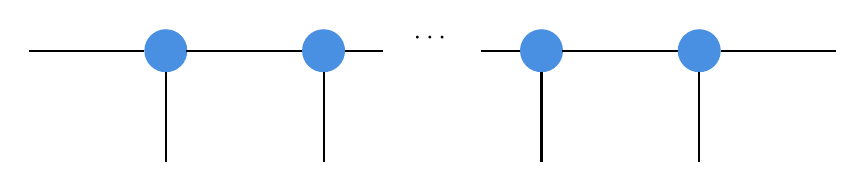
\begin{tikzpicture}[x=0.75pt,y=0.75pt,yscale=-1,xscale=1]
%uncomment if require: \path (0,300); %set diagram left start at 0, and has height of 300

%Straight Lines [id:da3529828319821786] 
\draw    (100,121) -- (155.71,121) ;
%Shape: Circle [id:dp4966257648856902] 
\draw  [draw opacity=0][fill={rgb, 255:red, 74; green, 144; blue, 226 }  ,fill opacity=1 ] (155.71,121) .. controls (155.71,115.28) and (160.34,110.65) .. (166.06,110.65) .. controls (171.78,110.65) and (176.41,115.28) .. (176.41,121) .. controls (176.41,126.72) and (171.78,131.35) .. (166.06,131.35) .. controls (160.34,131.35) and (155.71,126.72) .. (155.71,121) -- cycle ;
%Straight Lines [id:da5097517964421374] 
\draw    (166.06,131.35) -- (166.06,174.47) ;
%Straight Lines [id:da5757875200950937] 
\draw    (176,121) -- (231.71,121) ;
%Shape: Circle [id:dp31753487336843933] 
\draw  [draw opacity=0][fill={rgb, 255:red, 74; green, 144; blue, 226 }  ,fill opacity=1 ] (231.71,121) .. controls (231.71,115.28) and (236.34,110.65) .. (242.06,110.65) .. controls (247.78,110.65) and (252.41,115.28) .. (252.41,121) .. controls (252.41,126.72) and (247.78,131.35) .. (242.06,131.35) .. controls (236.34,131.35) and (231.71,126.72) .. (231.71,121) -- cycle ;
%Straight Lines [id:da5499396691584562] 
\draw    (242.06,131.35) -- (242.06,174.47) ;
%Shape: Circle [id:dp46956631085551503] 
\draw  [draw opacity=0][fill={rgb, 255:red, 74; green, 144; blue, 226 }  ,fill opacity=1 ] (336.71,121) .. controls (336.71,115.28) and (341.34,110.65) .. (347.06,110.65) .. controls (352.78,110.65) and (357.41,115.28) .. (357.41,121) .. controls (357.41,126.72) and (352.78,131.35) .. (347.06,131.35) .. controls (341.34,131.35) and (336.71,126.72) .. (336.71,121) -- cycle ;
%Straight Lines [id:da05730224870138678] 
\draw    (347.06,131.35) -- (347.06,174.47) ;
%Straight Lines [id:da830776528549658] 
\draw    (357,121) -- (412.71,121) ;
%Shape: Circle [id:dp008803468324955599] 
\draw  [draw opacity=0][fill={rgb, 255:red, 74; green, 144; blue, 226 }  ,fill opacity=1 ] (412.71,121) .. controls (412.71,115.28) and (417.34,110.65) .. (423.06,110.65) .. controls (428.78,110.65) and (433.41,115.28) .. (433.41,121) .. controls (433.41,126.72) and (428.78,131.35) .. (423.06,131.35) .. controls (417.34,131.35) and (412.71,126.72) .. (412.71,121) -- cycle ;
%Straight Lines [id:da019733050780630812] 
\draw    (423.06,131.35) -- (423.06,174.47) ;
%Straight Lines [id:da7512416171551617] 
\draw    (433.41,121) -- (489.12,121) ;
%Straight Lines [id:da28870663678175323] 
\draw    (252.41,121) -- (270.71,121) ;
%Straight Lines [id:da6449842400542742] 
\draw    (317.71,121) -- (336.71,121) ;

% Text Node
\draw (284,110.4) node [anchor=north west][inner sep=0.75pt]    {$\cdots $};


\end{tikzpicture}

    \caption{MPS拟设,根据不同的边界条件可以调整最左边和最右边两个外线;向下的线连接每个格点上的基矢量}
    \label{fig:mps-state}
\end{figure}

\subsubsection{旧式DMRG}

我们首先来实现海森堡模型的旧式的、真的根据约化密度矩阵决定保留哪些能量本征态的DMRG。算法如下:


\subsubsection{MPS方法}

现在我们转而使用更加现代的方式理解海森堡模型的DMRG。

\begin{figure}
    \centering
    

\tikzset{every picture/.style={line width=0.75pt}} %set default line width to 0.75pt        

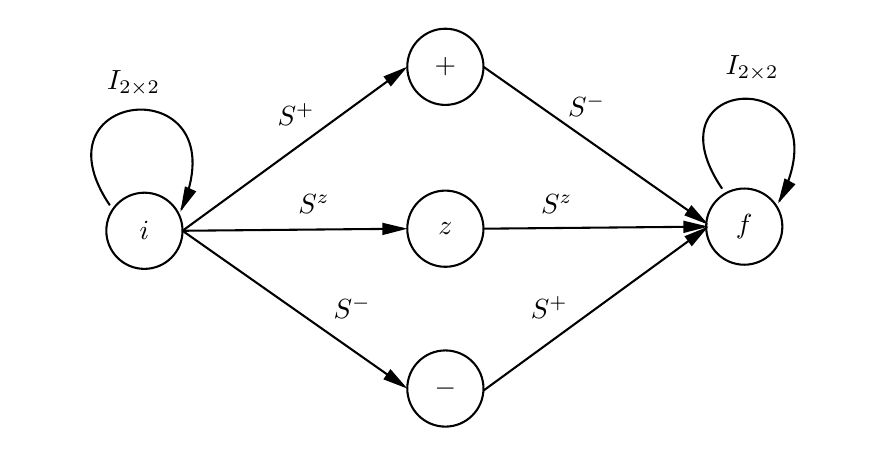
\begin{tikzpicture}[x=0.75pt,y=0.75pt,yscale=-1,xscale=1]
%uncomment if require: \path (0,328); %set diagram left start at 0, and has height of 328

%Shape: Circle [id:dp19428107127030758] 
\draw   (252,96.35) .. controls (252,86.22) and (260.22,78) .. (270.35,78) .. controls (280.49,78) and (288.71,86.22) .. (288.71,96.35) .. controls (288.71,106.49) and (280.49,114.71) .. (270.35,114.71) .. controls (260.22,114.71) and (252,106.49) .. (252,96.35) -- cycle ;

%Shape: Circle [id:dp49492495568136396] 
\draw   (252,174.35) .. controls (252,164.22) and (260.22,156) .. (270.35,156) .. controls (280.49,156) and (288.71,164.22) .. (288.71,174.35) .. controls (288.71,184.49) and (280.49,192.71) .. (270.35,192.71) .. controls (260.22,192.71) and (252,184.49) .. (252,174.35) -- cycle ;
%Shape: Circle [id:dp604607054970826] 
\draw   (252,251.35) .. controls (252,241.22) and (260.22,233) .. (270.35,233) .. controls (280.49,233) and (288.71,241.22) .. (288.71,251.35) .. controls (288.71,261.49) and (280.49,269.71) .. (270.35,269.71) .. controls (260.22,269.71) and (252,261.49) .. (252,251.35) -- cycle ;
%Shape: Circle [id:dp6016992738545592] 
\draw   (107,175.35) .. controls (107,165.22) and (115.22,157) .. (125.35,157) .. controls (135.49,157) and (143.71,165.22) .. (143.71,175.35) .. controls (143.71,185.49) and (135.49,193.71) .. (125.35,193.71) .. controls (115.22,193.71) and (107,185.49) .. (107,175.35) -- cycle ;

%Shape: Circle [id:dp5168816052832117] 
\draw   (396,173.35) .. controls (396,163.22) and (404.22,155) .. (414.35,155) .. controls (424.49,155) and (432.71,163.22) .. (432.71,173.35) .. controls (432.71,183.49) and (424.49,191.71) .. (414.35,191.71) .. controls (404.22,191.71) and (396,183.49) .. (396,173.35) -- cycle ;

%Curve Lines [id:da004973641561244246] 
\draw    (108.71,163.08) .. controls (69.61,105.45) and (172.67,97.16) .. (143.16,165.05) ;
\draw [shift={(142.71,166.08)}, rotate = 294.19] [fill={rgb, 255:red, 0; green, 0; blue, 0 }  ][line width=0.08]  [draw opacity=0] (12,-3) -- (0,0) -- (12,3) -- cycle    ;
%Straight Lines [id:da1995371487826203] 
\draw    (143.71,175.35) -- (250.38,97.53) ;
\draw [shift={(252,96.35)}, rotate = 503.89] [fill={rgb, 255:red, 0; green, 0; blue, 0 }  ][line width=0.08]  [draw opacity=0] (12,-3) -- (0,0) -- (12,3) -- cycle    ;
%Straight Lines [id:da3411444830583379] 
\draw    (143.71,175.35) -- (250.36,250.2) ;
\draw [shift={(252,251.35)}, rotate = 215.06] [fill={rgb, 255:red, 0; green, 0; blue, 0 }  ][line width=0.08]  [draw opacity=0] (12,-3) -- (0,0) -- (12,3) -- cycle    ;
%Straight Lines [id:da19216119538242293] 
\draw    (143.71,175.35) -- (250,174.37) ;
\draw [shift={(252,174.35)}, rotate = 539.47] [fill={rgb, 255:red, 0; green, 0; blue, 0 }  ][line width=0.08]  [draw opacity=0] (12,-3) -- (0,0) -- (12,3) -- cycle    ;
%Straight Lines [id:da07249965960790683] 
\draw    (288.71,174.35) -- (395,173.37) ;
\draw [shift={(397,173.35)}, rotate = 539.47] [fill={rgb, 255:red, 0; green, 0; blue, 0 }  ][line width=0.08]  [draw opacity=0] (12,-3) -- (0,0) -- (12,3) -- cycle    ;
%Straight Lines [id:da2874892398213533] 
\draw    (288.71,96.35) -- (395.36,171.2) ;
\draw [shift={(397,172.35)}, rotate = 215.06] [fill={rgb, 255:red, 0; green, 0; blue, 0 }  ][line width=0.08]  [draw opacity=0] (12,-3) -- (0,0) -- (12,3) -- cycle    ;
%Straight Lines [id:da20880092934159666] 
\draw    (288.71,252.35) -- (395.38,174.53) ;
\draw [shift={(397,173.35)}, rotate = 503.89] [fill={rgb, 255:red, 0; green, 0; blue, 0 }  ][line width=0.08]  [draw opacity=0] (12,-3) -- (0,0) -- (12,3) -- cycle    ;
%Curve Lines [id:da43441994643103965] 
\draw    (403.71,155.08) .. controls (364.61,97.45) and (465.69,95.1) .. (431.24,161.08) ;
\draw [shift={(430.71,162.08)}, rotate = 298.25] [fill={rgb, 255:red, 0; green, 0; blue, 0 }  ][line width=0.08]  [draw opacity=0] (12,-3) -- (0,0) -- (12,3) -- cycle    ;

% Text Node
\draw (270.35,96.35) node    {$+$};
% Text Node
\draw (125.35,175.35) node    {$i$};
% Text Node
\draw (414.35,173.35) node    {$f$};
% Text Node
\draw (120.16,111.78) node [anchor=south] [inner sep=0.75pt]    {$I_{2\times 2}$};
% Text Node
\draw (418.16,104.78) node [anchor=south] [inner sep=0.75pt]    {$I_{2\times 2}$};
% Text Node
\draw (188,112.4) node [anchor=north west][inner sep=0.75pt]    {$S^{+}$};
% Text Node
\draw (310,205.4) node [anchor=north west][inner sep=0.75pt]    {$S^{+}$};
% Text Node
\draw (270.35,174.35) node    {$z$};
% Text Node
\draw (270.35,251.35) node    {$-$};
% Text Node
\draw (328,108.4) node [anchor=north west][inner sep=0.75pt]    {$S^{-}$};
% Text Node
\draw (215,205.4) node [anchor=north west][inner sep=0.75pt]    {$S^{-}$};
% Text Node
\draw (198,156.4) node [anchor=north west][inner sep=0.75pt]    {$S^{z}$};
% Text Node
\draw (315,156.4) node [anchor=north west][inner sep=0.75pt]    {$S^{z}$};


\end{tikzpicture}

    \caption{海森堡模型的哈密顿量对应的自动机}
    \label{fig:heisenberg-automata}
\end{figure}

我们还需要将哈密顿量也写成张量网络的形式。一维的足够局域的系统的哈密顿量总是可以写成矩阵乘积算符的形式。
海森堡模型的哈密顿量可以看成一系列形如
\[
    \cdots \otimes I \otimes S^z \otimes S^z \otimes I \otimes \cdots
\]
或
\[
    \cdots \otimes I \otimes S^+ \otimes S^- \otimes I \otimes \cdots
\]
或
\[
    \cdots \otimes I \otimes S^- \otimes S^+ \otimes I \otimes \cdots
\]
的项的和。这种连乘的序列可以使用\autoref{fig:heisenberg-automata}所示的自动机描述。
这个自动机的状态有五种,依次是$f, -, +, z, i$(排列顺序和转移矩阵\eqref{eq:heisenberg-mpo-transition-matrix}的矩阵元对应的基底的顺序一致)。
海森堡模型中的任意一个直积序列都可以由这个自动机产生,而它也只产生海森堡模型哈密顿量中的直积序列。
转移矩阵为
\begin{equation}
    \pmqty{
        I_{2 \times 2} & 0 & 0 & 0 & 0 \\
        S^+ & 0 & 0 & 0 & 0 \\
        S^- & 0 & 0 & 0 & 0 \\
        S^z & 0 & 0 & 0 & 0 \\
        0 & S^- & S^+ & S^z & I_{2 \times 2}
    }
    \label{eq:heisenberg-mpo-transition-matrix}
\end{equation}
的自动机产生。
。
将\eqref{eq:heisenberg-mpo-transition-matrix}连乘$N$次,其矩阵元的乘法视为直积,则最终得到的转移矩阵中对应$i \to f$的矩阵元就是海森堡模型的哈密顿量。
注意\eqref{eq:heisenberg-mpo-transition-matrix}实际上有四个指标,将两个\eqref{eq:heisenberg-mpo-transition-matrix}相乘无非是将不涉及$I_{2 \times 2}, S^+, S^-, S^z$内部结构的两个指标缩并,于是以\eqref{eq:heisenberg-mpo-transition-matrix}为四阶张量构造如下张量网络
\[
    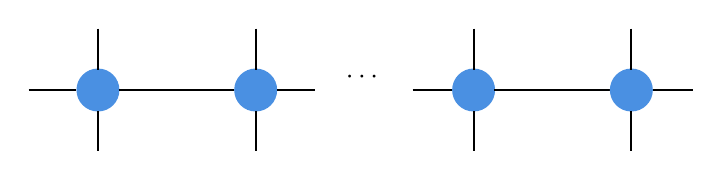
\begin{tikzpicture}[x=0.75pt,y=0.75pt,yscale=-1,xscale=1]
        %uncomment if require: \path (0,300); %set diagram left start at 0, and has height of 300
        
        %Straight Lines [id:da3529828319821786] 
        \draw    (132.71,121) -- (155.71,121) ;
        %Shape: Circle [id:dp4966257648856902] 
        \draw  [draw opacity=0][fill={rgb, 255:red, 74; green, 144; blue, 226 }  ,fill opacity=1 ] (155.71,121) .. controls (155.71,115.28) and (160.34,110.65) .. (166.06,110.65) .. controls (171.78,110.65) and (176.41,115.28) .. (176.41,121) .. controls (176.41,126.72) and (171.78,131.35) .. (166.06,131.35) .. controls (160.34,131.35) and (155.71,126.72) .. (155.71,121) -- cycle ;
        %Straight Lines [id:da5097517964421374] 
        \draw    (166.06,131.35) -- (166.06,150.47) ;
        %Straight Lines [id:da5757875200950937] 
        \draw    (176,121) -- (231.71,121) ;
        %Shape: Circle [id:dp31753487336843933] 
        \draw  [draw opacity=0][fill={rgb, 255:red, 74; green, 144; blue, 226 }  ,fill opacity=1 ] (231.71,121) .. controls (231.71,115.28) and (236.34,110.65) .. (242.06,110.65) .. controls (247.78,110.65) and (252.41,115.28) .. (252.41,121) .. controls (252.41,126.72) and (247.78,131.35) .. (242.06,131.35) .. controls (236.34,131.35) and (231.71,126.72) .. (231.71,121) -- cycle ;
        %Straight Lines [id:da5499396691584562] 
        \draw    (242.06,131.35) -- (242.06,150.47) ;
        %Shape: Circle [id:dp46956631085551503] 
        \draw  [draw opacity=0][fill={rgb, 255:red, 74; green, 144; blue, 226 }  ,fill opacity=1 ] (336.71,121) .. controls (336.71,115.28) and (341.34,110.65) .. (347.06,110.65) .. controls (352.78,110.65) and (357.41,115.28) .. (357.41,121) .. controls (357.41,126.72) and (352.78,131.35) .. (347.06,131.35) .. controls (341.34,131.35) and (336.71,126.72) .. (336.71,121) -- cycle ;
        %Straight Lines [id:da05730224870138678] 
        \draw    (347.06,131.35) -- (347.06,150.47) ;
        %Straight Lines [id:da830776528549658] 
        \draw    (357,121) -- (412.71,121) ;
        %Shape: Circle [id:dp008803468324955599] 
        \draw  [draw opacity=0][fill={rgb, 255:red, 74; green, 144; blue, 226 }  ,fill opacity=1 ] (412.71,121) .. controls (412.71,115.28) and (417.34,110.65) .. (423.06,110.65) .. controls (428.78,110.65) and (433.41,115.28) .. (433.41,121) .. controls (433.41,126.72) and (428.78,131.35) .. (423.06,131.35) .. controls (417.34,131.35) and (412.71,126.72) .. (412.71,121) -- cycle ;
        %Straight Lines [id:da019733050780630812] 
        \draw    (423.06,131.35) -- (423.06,150.47) ;
        %Straight Lines [id:da7512416171551617] 
        \draw    (433.41,121) -- (452.71,121) ;
        %Straight Lines [id:da28870663678175323] 
        \draw    (252.41,121) -- (270.71,121) ;
        %Straight Lines [id:da6449842400542742] 
        \draw    (317.71,121) -- (336.71,121) ;
        %Straight Lines [id:da7841710435675986] 
        \draw    (166.06,91.47) -- (166.06,111.47) ;
        %Straight Lines [id:da17804726526071146] 
        \draw    (242.06,91.47) -- (242.06,111.47) ;
        %Straight Lines [id:da7740864916724297] 
        \draw    (347.06,91.47) -- (347.06,111.47) ;
        %Straight Lines [id:da6302856555632439] 
        \draw    (423.06,91.47) -- (423.06,111.47) ;
        
        % Text Node
        \draw (284,110.4) node [anchor=north west][inner sep=0.75pt]    {$\cdots $};
        \end{tikzpicture}        
\]
就得到了哈密顿量,或者说得准确一些,哈密顿量在$\{S^z_i\}$表象下的矩阵元。

\begin{info}{张量网络库}{tensor-network-libs}
    Julia语言的iTensor库(见\cite{itensor})提供了指标可命名(从而无需特别注意指标顺序)的张量,张量可以使用基于量子数的稀疏矩阵存储,可用于快速编写张量网络程序。
    iTensor也提供了许多有用的通用工具,使用很短的代码即可实现DMRG。
    
    APLS是一个含有各种计算物理方法的C++库。
\end{info}

\section{横场伊辛模型}

\subsection{张量网络模拟}

\chapter{自旋玻璃}

\concept{自旋玻璃}是一类自旋之间的相互作用随机的自旋系统,由于自旋间相互作用随机,无法形成自旋的长程序,从而,每个局部的自旋看起来都是稳定地冻结了的,即形成了短程序,然而无法定义任何长程的序参量,因为相邻的短程序的指向各不相同;相应的,系统存在一系列亚稳态,它们的能量彼此相差不多,从而如果系统构型落入了其中一个亚稳态,它可以在其中停留足够长的时间。
这种大量实际上非常稳定的亚稳态存在,有短程序而没有长程序的物态和玻璃非常相似,这也就是我们称它为自旋玻璃的原因。

\section{Edwards–Anderson模型}

